\documentclass[]{article}

\usepackage{enumerate}
\usepackage{amssymb}
\usepackage{graphicx}
\usepackage{ulem}

\def\OR{\vee}
\def\AND{\wedge}
\def\imp{\rightarrow}
\def\math#1{$#1$}
\def\mand#1{$$#1$$}
\def\mld#1{\begin{equation}
#1
\end{equation}}
\def\eqar#1{\begin{eqnarray}
#1
\end{eqnarray}}
\def\eqan#1{\begin{eqnarray*}
#1
\end{eqnarray*}}
\def\cl#1{{\cal #1}}

\DeclareSymbolFont{AMSb}{U}{msb}{m}{n}
\DeclareMathSymbol{\N}{\mathbin}{AMSb}{"4E}
\DeclareMathSymbol{\Z}{\mathbin}{AMSb}{"5A}
\DeclareMathSymbol{\R}{\mathbin}{AMSb}{"52}
\DeclareMathSymbol{\Q}{\mathbin}{AMSb}{"51}
\DeclareMathSymbol{\I}{\mathbin}{AMSb}{"49}
\DeclareMathSymbol{\C}{\mathbin}{AMSb}{"43}

\begin{document}
\bf \Large Gabriel Maayan - FOCS Assignment 3

\section{DMC 13.3}
There are two cases:
\begin{enumerate}[(1)]
\item Start with a hot meal. Then there are two options for breakfast, one for lunch, and two for dinner. This gives a total of four options.
\item Start with a cold meal. There are two options for breakfast, two for lunch, and two for dinner, giving eight options.
\end{enumerate}
In total, this gives 12 options for daily menus.

\section{DMC 13.4}
Let each day be a digit in a binary sequence. A day where you walk a mile is a \math{1} and a day where you sleep in is a \math{0}. 
This gives a binary sequence of length 20, with 12 one's. The number of combinations is \math{(_{12}^{20}) = 125970} possible ways 
to walk 12 miles in 20 days.

\section{DMC 13.20}
\begin{enumerate}[(c)]
\item The total number of ways to make the digits add up to 27 is \math{(_5^{32})}, but that includes digits that are larger than 9, so 
subtracting those cases and adding back in the ones that were correct, you get \math{(_5^{32})-(_1^6)(_5^{22})+(_5^{12})(_2^6)=55252} possible ways.


\end{enumerate}

\section{DMC 13.40}
\math{x_1=z_1, x_2=z_2-z_1, \cdots , x_k=z_k-z_{k-1}\\
x_1+x_2+\cdots +x_k=\sout{z_1}+\sout{z_2}-\sout{z_1}+\cdots+z_k-\sout{z_{k-1}}=z_k\leq n \\}
Gives a sequence of length \math{n+k} with \math{k} ones, so the number of sequences is \math{(_k^{n+k})}.

\section{DMC 14.32}
\begin{enumerate}[(a)]
\item 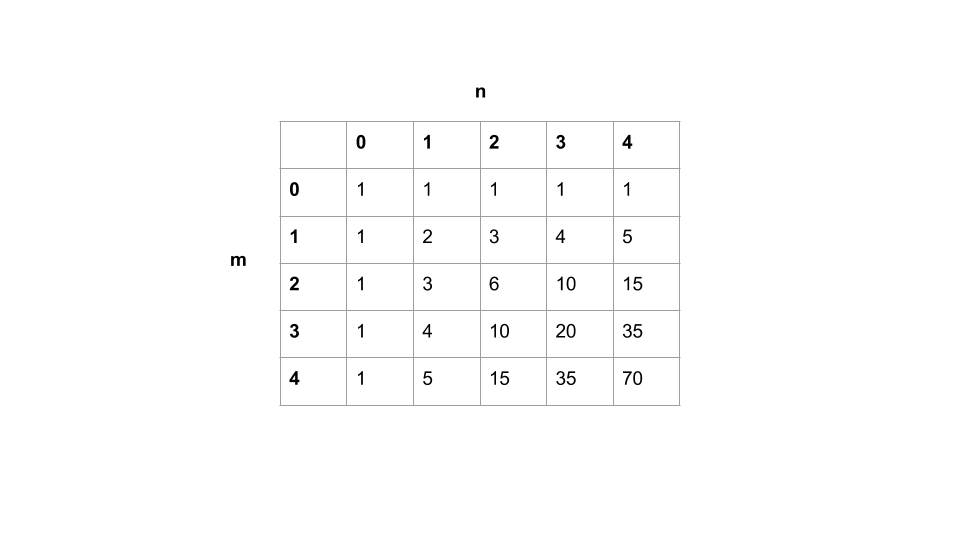
\includegraphics[width=\linewidth]{HW7a}
As shown by the table, any number is the sum of the number above it and the number to the right of it. Thus, 
\math{P(n, m) = P(n, m-1) + P(n-1, m)}

\item Also shown by the table above, \math{P(0, m) = P(n, 0) = 1}.

\item As seen in the table, \math{P(4, 4) = 70}.

\item A diagonal on the table cooresponds to a row in Pascal's triangle. For instance, the second diagonal is the 
same as the second row in Pascal's triangle. The constant on a diagonal is \math{n+m}, so \math{n_p = n+m}, 
and \math{k_p = n}. Therefore, \math{P(n, m) = (_n^{n+m})}.

\item 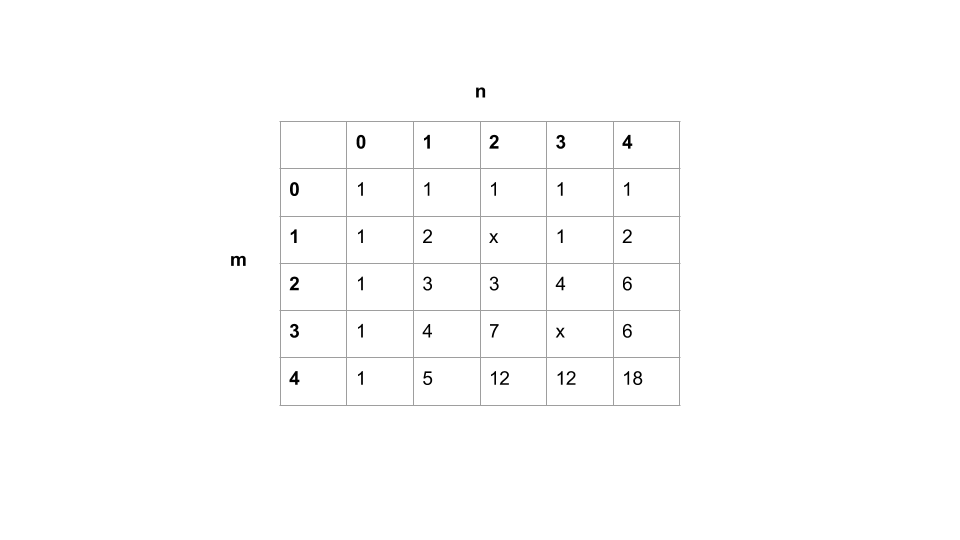
\includegraphics[width=\linewidth]{HW7b}
 The new table would look like the above table, so the new \math{P(4, 4) = 18}.

\item The number of combinations is equal to the ways to get to \math{(4, 4)}, minus the ways to get to the crossed 
off spaces, plus the ways to get to the spaces in the middle. This is \math{(_4^8) - (_1^3)(_2^3) - (_3^6)(_1^2) + (_1^3)(_1^3)(_1^2)}.

\end{enumerate}

\section{DMC 12.19}
By Theorem 12.4, there is a stable matching with a group of \math{n} men and \math{n} women. Suppose there is a group of \math{n} 
men and \math{n} women, that is in a stable matching. If any two men or any two women are switched, there is an unstable matching, 
because those matchings would prefer to switch back. 
Therefore, there does not exist an \math{n\geq 3} for which there are preferences of \math{n} men and \math{n} women such 
that every matching is stable.


\end{document}
